\documentclass[a4paper,12pt,one side,titlepage]{report}


%en francais
\usepackage[T1]{fontenc}
\usepackage{lmodern}
\usepackage[utf8]{inputenc}
\usepackage[francais]{babel}



\usepackage{listings}
\usepackage{geometry}
\usepackage{graphicx}
\usepackage{eurosym}
\usepackage{url}
\usepackage{pdfpages}
\usepackage[acronym]{glossaries}
\usepackage{hyperref}
\usepackage{graphicx}
%\usepackage[top=2.5cm,bottom=2.5cm,left=2.5cm,right=2.5cm]{geometry}
%\hypersetup{pdfborder=0}




\newglossaryentry{firewall}
{
	name={firewall},
	description={Protection pour serveur}
}

\newglossaryentry{naxsi}
{
	name={naxsi},
	description={Un type de firewall}
}



\makeglossaries
\begin{document}
%\includepdf[pages = {1-1}]{./pdf/1stpage.pdf}
%\includepdf[pages = {1-1}]{./pdf/pagegarde.pdf}


\begin{titlepage}
\begin{center}

\textsc{\LARGE Licence ASRALL}\\[1.5cm]

\textsc{\Large Exposé technique}\\[5.9cm]

% Title
{ \huge \bfseries Fully Automatic Installation\\[1.9cm] }

% Author and supervisor
\noindent
\begin{minipage}{0.4\textwidth}
\begin{flushleft} \large
François \textsc{Dupont}
\end{flushleft}
\end{minipage}%
\begin{minipage}{0.4\textwidth}
\begin{flushright} \large
Florent \textsc{Fillion}
\end{flushright}
\end{minipage}

\vfill

% Bottom of the page
{\large \today}

\end{center}
\end{titlepage}


%Page table des matières
\tableofcontents

%Introduction
\chapter{Introduction}
\section{Objectifs}
\subsection{Définition}
\textit{Fully Automatic Installation} ou \textsc{FAI} est un logiciel libre, inspiré de son équivalent \textsc{Solaris}, \textsc{Jumpstart}. Il permet d'installer et de configurer un système d'exploitation Linux sur une ou plusieurs machines, en utilisant un infrastructure client serveur, de façon rapide et automatisé.

Il est à noter que \textsc{FAI} n'est pas interactif contrairement à d'autres logiciels remplissant sensiblement la même fonction. Ce logiciel est également considéré comme mature puisqu'il en est à sa 4\textsuperscript{ème} itération majeure (4.0) et est développé de façon continue depuis 1999.
\textsc{FAI} est également très bien documenté, documentation disponible sous de multiple formats, avec un outil de recherche très efficace

\subsection{Utilité}
\textsc{FAI} s'adresse particulièrement aux administrateurs ayant à gérer un grand parc de machine sous Linux, que ce parc soit \textit{virtualisé} ou physique (et même des \textit{chroot}s).

\section{Histoire}
\textsc{FAI} est née en 1999 alors que Thomas \textsc{Lange}, Administrateur système experimenté sur Solaris a dû déployer plusieurs machines Debian/Gnu/Linux. Comme tous les administrateurs \textit{(compétents?)}, il déteste réaliser des choses répétitives et décide donc de s'atteler à l'automatisation du déploiement de machines Debian. Son projet est un succès, et est maintenant utilisé par de nombreuses administrations, écoles et entreprises.
Il est également, depuis, devenu développeur Debian.

Il a depuis été rejoint par d'autres développeurs, notamment Michael \textsc{Prokop} également développeur Debian et aussi mainteneur du dérivé minimaliste et orienté pour l'administration système \textsc{Grml}.
Et par Kerim \textsc{Gueney} collègue de \textsc{Lange} à l'Université de Cologne.

On peut remarquer que ce projet est particulièrement basé en Allemagne, cependant sa documentation (bien qu'actuellement non à jour) est disponible en Anglais.



\section{Concepts}
Cette partie pourrait avoir sa place dans le chapitre traitant de la technique à proprement parler, cependant, il nous semble essentiel d'exposer les principes fondamentaux (et simples une fois assimilés) de \textsc{FAI}. Il s'agit ici d'un survol, plus d'informations seront disponibles dans la partie réservé à la technique.

\subsection{Architecture Client Serveur}
Il est important de comprendre que \textsc{FAI} ne fonctionne qu'en mode client serveur (et pas par exemple en pair à pair). Avec 1 serveur pour N clients. Il est possible d'avoir plusieurs configurations clients disponibles, par exemple installer Debian stable sur certains type de machine et Debian unstable sur d'autres. 


\subsection{L'installation}
Le processus d'installation est assez simple : le client est éveillé par un quelconque moyen (USB, CD, PXE), il se connecte ensuite au serveur (cela nécessite d'avoir un réseau fonctionnel (DHCP). Notre client monte ensuite un partage NFS présent sur le serveur comme sa racine, une fois le noyau chargé, le script script d'installation FAI suit son court et installe les configurations demandées par l'administrateur. Ce/Ces scripts peuvent inclure un partitionnement des disques ou bien formatage, l'installation de logiciels spécifique, gestion du RAID materiel, etc...

\subsection{La configuration}
Comme expliqué précedemment il est possible d'avoir une grande variété de configuration différentes. Mais il est possible d'utiliser un système de classe (programmation) pour créer des groupes d'ordinateurs similaires et ainsi facilité l'industrialisation de notre installation (il serait contre productif d'avoir à un profil par client). Il est possible d'utiliser plusieurs langages pour réaliser les scripts, bash, perl, ruby.

\chapter{Technique}

\section{Préparer et installer FAI}

\section{Le processus d'installation}

\section{Mon premier boot}

\section{Quid des architectures}

\section{Installer autre chose que Debian}

\section{Les updates}

\chapter{Alternatives}
Il existe plusieurs alternatives à FAI, tels que Jumpstart(Solaris), Kickstart(RedHat), Rembo, ou encore ...................

\section{Jumpstart}
......................

\section{Kickstart}
Kickstart a été créé par RedHat afin d'automatiser l'installation de Fedora et Red Hate Enterprise Linux. Sa configuration s'effectue dans un fichier texte unique contenant une liste d'éléments, chacun identifié par un mot-clé. Ces éléments correspondent aux réponses à toutes les questions qui devraient normalement être posées lors d'une installation typique.\\
Ce fichier peut être créé manuellement en partant d'un fichier vierge puis en écrivant les directives une par une.
Cependant, et contrairement à FAI, il existe une interface utilisateur graphique, "Kickstart Configuration", permettant ainsi une configuration plus simple puisque il n'est pas nécessaire de se rappeler de la syntaxe exacte des fichiers :\\
\begin{center}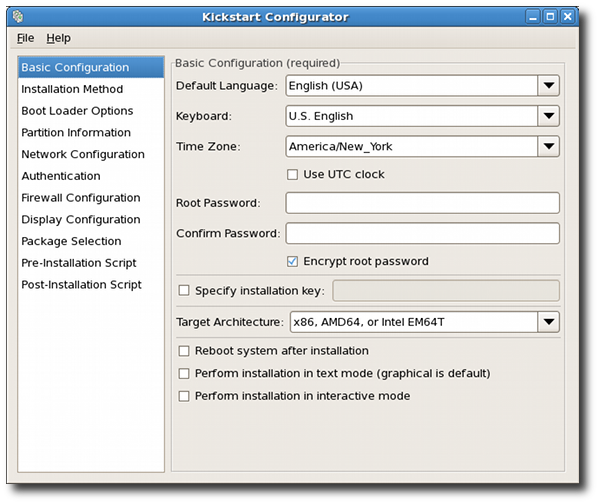
\includegraphics[scale=0.5]{./img/kickstart.png}\end{center}
.......................

\section{Rembo}
Rembo est le successeur de BPBatch. C’est un environnement commercial de création et de déploiement d’images sur PC. Le serveur Rembo peut s’exécuter sur Windows, Linux, ou encore FreeBSD et s’appuie sur un serveur DHCP. Les machines clientes doivent donc supporter PXE. Les clients du réseau sont répartis en plusieurs groupes, ce qui permet de définir des comportements par type de machine, par salle, ... 

\chapter{Sources}
http://fai-project.org/\\
http://www.markus-gattol.name/ws/fai.html\\
https://github.com/faiproject/fai\\
https://www.linux-magazine.com/w3/issue/100/066-071\_FAI.pdf\\
http://grml.org/\\

\end{document}
